% -*-coding: utf-8;-*-
%\section{Описание программного пакета}

\subsection{Основные решаемые задачи}\label{main_tasks}

В соответствии со своим назначением программный пакет должен решать
задачи моделирования САУ, моделирования и обучения нейронных сетей.
Типовой сеанс работы с пакетом подразумевает интерактивное
взаимодействие пользователя с программами.  Поскольку пакет
разрабатывается для применения в учебном процессе, весьма желательно,
чтобы он был:
\begin{itemize}
\item простым в изучении и использовании;
\item адаптированным к специфике учебного процесса;
\item быстродействующим на не самых современных компьютерах;
\item открытым к модификации;
\item основанным на общедоступных и открытых технологиях.
\end{itemize}

При моделировании систем автоматического управления необходимо
предусмотреть возможность гибкой настройки контура и условий его
работы.  В частности, должны настраиваться:
\begin{itemize}
\item уставка (стохастическая, детерминированная);
\item помеха (стохастическая, детерминированная);
\item регулятор (линейный, нейросетевой);
\item объект управления (линейный, нелинейный, нестационарный).
\end{itemize}

%TODO: аргументировать, почему эти свойства важны.  м.б., в первой главе

В то же время, учитывая учебную направленность пакета, представляется
достаточным ограничиться одноконтурными системами управления когда
объект является одноканальным по входу и выходу.  Это существенно
упрощает интерактивную часть пакета и практику его использования.

Для моделирования и обучения нейронных сетей должны иметься следующие
возможности:
\begin{itemize}
\item создание нейронной сети с произвольной архитектурой в классе
  многослойных персептронов;
\item обучение нейронной сети на заданной выборке с контролем процесса
  по тестовой выборке;
\item предсказание поведения объекта управления с помощью нейронной
  сети в контуре в процессе моделирования;
\item обучение нейронной сети регулятора в контуре управления в
  процессе его моделирования.
\end{itemize}

Специфика применения нейронных сетей в системах автоматического
управления заключается в преимущественном использовании сетей класса
``многослойный персептрон'' с обучением методом обратного
распространения или более эффективными его вариантами.  По этой
причине нецелесообразно реализовывать поддержку сетей существенно иных
парадигм (Кохонена, Хопфилда и пр.).  Иногда применяемые в САУ
нейронные сети, основанные на радиально-базисных функциях (RBF),
доказанно являются эквивалентными многослойному персептрону, поэтому
их реализация тоже является избыточной и ради простоты программного
комплекса от неё целесообразно отказаться.

%\subsection{Структура пакета и выбор инструментария}
\subsection{Структура пакета и инструментальные средства}

Анализ требований к пакету обнаруживает, что некоторые из них трудно
совместить, пользуясь какой-то одной инструментальной технологией
разработки программ.  В частности, эффективное выполнение
вычислительных алгоритмов требует компиляции программ перед
выполнением.  Только с помощью компиляции можно обеспечить приемлемое
быстродействие на не всегда современных компьютерах, используемых в
учебном процессе.  В то же время, открытость к модификации
подразумевает возможность изменения программы прямо перед выполнением,
что важно для быстрой разработки, а также при углубленном изучении
пакета программ и проведении исследований с его помощью.

Кроме того, не все технологии разработки программного обеспечения
доступны на всех распространенных операционных системах: Microsoft
Windows, Linux, Mac OS X.  Некоторые из подходящих технологий
реализованы только в проприетарных программных продуктах,
использование которых требует покупки дорогостоящей лицензии.

В \tablref{tabl:sdk_tech} приводятся данные о сравнении нескольких
различных современных технологий разработки программного обеспечения
по перечисленным трем критериям.  Под технологиями в данном случае
понимается совокупность языка программирования, среды разработки и
выполнения и необходимые средства для реализации пользовательского
интерфейса и интерактивной графики.

\begin{table}[ht]
\centering
\caption{Сравнение технологий разработки программ.}
\label{tabl:sdk_tech}
\begin{tabular}{|l|c|c|c|}
\hline
\bf Технология & \bf Быстродействие & \bf Открытость к & \bf Общедоступность \\
             &                & \bf модификации  & \bf и открытость \\
\hline
             &                &  плохо       &              \\
\tt C++      &   отлично      & (требуется   & отлично      \\
             &                & компиляция)  &              \\
\hline
             &   средне       &  плохо       &              \\
\tt Java     & (интерпретация & (требуется   & отлично      \\
             & байт-кода)     & компиляция)  &              \\
\hline
             &   средне       &  плохо       & плохо        \\
\tt C$\#$    & (нужно много   & (требуется   & (в основном, \\
             & ресурсов)      & компиляция)  & для MS Windows) \\
\hline
            &   плохо        &              & средне       \\
\tt Python  & (интерпретация & отлично      & (нет унифициро- \\
            & байт-кода)     &              & ванной графики) \\
\hline
           &   плохо        &              &              \\
\tt Tcl/Tk & (интерпретация & отлично      & отлично      \\
           & байт-кода)     &              &              \\
\hline
           &   средне       &              & плохо        \\
\tt Matlab & (интерпретация & отлично      & (платный и   \\
           & байт-кода)     &              & очень дорогой) \\
\hline
\end{tabular}
\end{table}

Отсутствие идеальной технологии для разработки пакета моделирования и
нейросетевого управления вынуждает искать компромиссное решение.
Можно функционально разделить пакет на интерактивную и вычислительную
части и реализовать каждую с помощью оптимальной технологии.
Вычислительная часть требует эффективной реализации с точки зрения
быстродействия, поэтому целесообразно реализовать её на языке {\tt
  C++}.  Компиляторы этого языка программирования доступны для всех
значимых платформ, а сам язык, пожалуй, является в настоящее время
наиболее популярным среди универсальных процедурных языков
программирования.

Интерактивную графику и управление вычислительными алгоритмами важно
сделать максимально гибкими и открытыми для модификации.  Хорошим
выбором будет использование интерпретируемого языка с встроенными
возможностями для реализации пользовательского интерфейса, прикладной
графики и средствами интеграции программного обеспечения.  Одним из
подходящих инструментов является {\tt Tcl/Tk}, доступный бесплатно и в
исходных текстах для всех распространенных операционных систем.

Функциональная декомпозиция разрабатываемого пакета по используемым
технологиям разработки программ находит отражение в структуре
взаимодействия отдельных частей программного комплекса, которая
приводится на \figref{fig:prog_interaction_struct}.  Реализация
вычислительных функций в отдельных узкоспециализированных программах,
написанных на языке {\tt C++}, позволит пользователю гибко управлять
их взаимодействием и во многих нестандартных случаях снизит
необходимость в модификации текстов на {\tt C++}.

\begin{figure}
\centerline{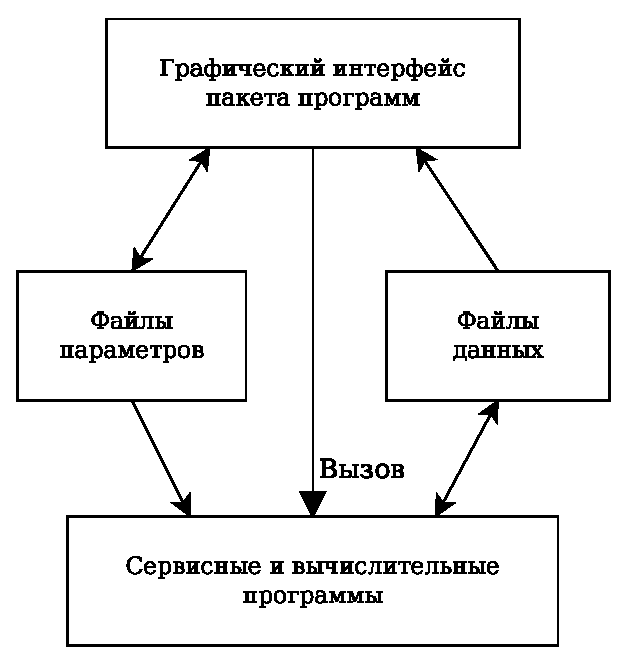
\includegraphics{princ_struct.eps}}
\caption{Схема взаимодействия частей программного пакета}
\label{fig:prog_interaction_struct}
\end{figure}

\subsection{Основные интерактивные элементы}

Интерактивная часть пакета разрабатывается с использованием парадигмы
событийно-управляемого программирования.  Действия пользователя
порождают события, которые, в свою очередь, приводят к вызову
процедур, ассоциированных с ними.  Структура событийно-управляемой
программы имеет следующие особенности:
\begin{itemize}
\item Основной структурирующей единицей программы является окно.
\item Перед появлением окна на экране выполняется программный код ---
  процедура инициализации окна, --- формирующий внешний вид и основные
  интерактивные возможности взаимодействия с этим окном.
\item Внешний вид окна и его поведение может зависеть от параметров
  процедуры инициализации.
\item Процедуры-обработчики событий устанавливаются при создании окна
  или в процессе его жизни.
\item Внешний вид окна и его поведение в течение жизни может зависеть
  от действий, выполняемых в тех или иных обработчиках сигналов.
\end{itemize}

В соответствии с поставленными задачами целесообразно распределить
функции программы между окнами пользовательского интерфейса со
следующим назначением:
\begin{enumerate}
\item моделирование системы автоматического управления включая случай
  нестационарного поведения объекта;
\item создание/просмотр/редактирование цепочки линейных и нелинейных
  звеньев;
\item создание/просмотр/редактирование нейронной сети;
\item обучение нейронной сети модели объекта управления с
  использованием указанных выборок вне контура;
\item обучение нейронной сети регулятора с использованием указанных
  выборок вне контура;
\item обучение нейронной сети регулятора в контуре управления в
  процессе его моделирования;
\item просмотр заданных выборок (дискретных временных рядов) в виде
  графиков по времени;
\item просмотр заданной выборки в виде гистограммы для оценки
  одномерного распределения;
\item просмотр двух заданных синхронных выборок в виде множества точек
  на двумерной плоскости для оценки двумерного распределения.
\end{enumerate}

\subsection{Сервисные и вычислительные программы}
% TODO: перечислить наименование и назначение ряда программ

В соответствии с разработанной схемой взаимодействия компонентов
пакета моделирования (\figref{fig:prog_interaction_struct}) основные
блоки, выполняющие численные расчеты и обработку данных, не связанную
непосредственно с визуализацией графики, реализуются на языке
программирования {\tt C++} набором неинтерактивных программ.  Эти
программы взаимодействуют друг с другом и с пользовательским
интерфейсом не непосредственно, а через файлы параметров и данных.

Управление работой программ поизводится путем задания всех необходимых
параметров перед их запуском.  В различных программах в зависимости от
сложности их параметризации реализованы следующие способы передачи
параметров:
\begin{itemize}
\item в качестве аргументов командной строки;
\item через переменные рабочего окружения;
\item через файл с параметрами.
\end{itemize}

Конфигурационные файлы с параметрами различных программ имеют общий
синтаксис, описанный в \tablref{tabl:par_syntax}.

\begin{table}[ht]
\centering
\caption{Описание формата файла параметров.}
\label{tabl:par_syntax}
\begin{tabular}{|c|l|p{10cm}|}
\hline
Правило & Синтаксис & Семантика \\
\hline
1 & \tt \#                 & Однострочный комментарий \\
2 & \tt \em Имя = Значение & Параметр с заданным именем и значением до конца строки \\
\hline
\end{tabular}
\end{table}

Перечень вычислительных и сервисных программ с классификацией по
областям назначения приведен в \tablref{tabl:prog_list}.

\begin{table}%[ht]
\centering
\caption{Список вычислительных и сервисных неинтерактивных программ пакета.}
\label{tabl:prog_list}
\begin{tabular}{|c|l|p{13cm}|}
\hline
$N^0$ & Название & Назначение \\
\hline
\hline
\multicolumn{3}{|c|}{Основные программы моделирования и специализированного обучения нейросетей} \\
\hline
1 & \tt dcsloop & Моделирование контура управления. \\
2 & \tt dplantid & Обучение нейросетевой модели объекта управления вне контура  \\
3 & \tt dnnplant & Проверка функционирования нейросетевой модели объекта \\
4 & \tt dcontrp & Предварительное обучение нейросетевого регулятора подобно заменяемому вне контура управления \\
5 & \tt dcontrf & Дообучение нейросетевого регулятора в контуре управления с помощью нейросетевой модели объекта \\
\hline
\multicolumn{3}{|c|}{Неспециализированная работа с нейронными сетями} \\
\hline
6 & \tt MakeNN & Подготовка файла нейронной сети заданной архитектуры \\
7 & \tt ResetNN & Инициализация весовых коэффициентов нейронной сети случайными значениями \\
8 & \tt TrainNN & Обучение нейронной сети общего вида на заданных примерах \\
9 & \tt EvalNN & Проверка работы настроенной нейронной сети общего вида \\
\hline
\multicolumn{3}{|c|}{Генерация временных рядов} \\
\hline
10 & \tt dmeander & Генерация временного ряда вида ``меандр'' \\
11 & \tt drand & Генерация случайного временного ряда с заданными параметрами \\
12 & \tt drandmea & Генерация случайного временного ряда вида ``меандр'' с заданными параметрами \\
13 & \tt dsin & Генерация моногармонического временного ряда с заданными параметрами \\
\hline
\multicolumn{3}{|c|}{Операции с временными рядами} \\
\hline
14 & \tt dmult & Умножение значений временного ряда на указанное число \\
15 & \tt dsub & Вычитание значений временных рядов \\
16 & \tt dsum & Сложение значений временных рядов \\
\hline
\multicolumn{3}{|c|}{Обработка и изучение временных рядов} \\
\hline
% & \tt d2ts & Нумерация значений временного ряда \\
17 & \tt dconst & Проверка гипотезы о постоянном среднем значении временного ряда \\
18 & \tt dcorr & Расчет функции корреляции указанной длины для заданных временных рядов \\
% & \tt djacob & Расчет дискретной оценки якобиана по временным рядам управляющего сигнала и состояния одномерного объекта \\
19 & \tt dmean & Расчет среднего значения временного ряда \\
20 & \tt dmse & Расчет среднеквадратичной ошибки временного ряда \\
% & \tt dsmooth & Сглаживание временного ряда на скользящей базе  \\
% & \tt dstat & Расчет статистических параметров временного ряда нарастающим итогом \\
% & \tt dstatsb & Расчет статистических параметров временного ряда в скользящей базе \\
21 & \tt dstddev & Расчет среднеквадратичного отклонения временного ряда \\
22 & \tt dtf & Применение заданной линейной передаточной или комбинированной функции к указанному временному ряду  \\
23 & \tt Distr1D & Построение одномерного распределения временного ряда \\
24 & \tt Distr2D & Построение двумерного распределения временного ряда \\
% & \tt FileCvt & Преобразование формата файла временного ряда \\
25 & \tt StatAn & Расчет статистических параметров временного ряда \\
\hline
\multicolumn{3}{|c|}{Алгоритм кумулятивных сумм} \\
\hline
26 & \tt acstest & Проверка параметров АКС вне контура управления \\
\hline
\end{tabular}
\end{table}


\subsection{Объектная библиотека}

Объектно-ориентированная библиотека {\tt NeuArch} разработана на языке
программирования {\tt C++} и предназначена для реализации следующих
основных задач:
\begin{enumerate}
\item Работа с цепочками линейных и нелинейных звеньев: создание,
  выполнение, хранение в файлах.
\item Работа с нейросетями архитектуры ``многослойный персептрон'':
  создание, обучение, выполнение, хранение в файлах.
\item Моделирование динамических систем в дискретном времени.
\end{enumerate}

Кроме того, библиотека реализует ряд необходимых вспомогательных
функций: ввод/вывод временных рядов, чтение и запись файлов
параметров, абстрактные структуры данных и прочий сервис.

Библиотека является переносимой (функционирует на ОС MS Windows и
Linux) и универсальной, то есть, не содержит буквальной реализации
высокоуровневых функций, возложенных на программный пакет.

\subsubsection{Моделирование линейных звеньев}

Для моделирования на компьютере системы управления в целом необходимо
иметь компьютерные модели составных элементов.  Для описания линейного
элемента удобно воспользоваться z-преобразованием передаточной
функции.  Это представление является общепринятым в классе линейных
систем в дискретном времени.

В программном пакете передаточная функция $P^*(z)$ линейного элемента
описывается произвольной комбинацией следующих базовых конструкций:

\begin{equation}\label{eq:polyfrac}
P^*(z)=\frac{a_nz^n+a_{n-1}z^{n-1}+...+a_0}{b_mz^m+b_{m-1}z^{m-1}+...+b_0}
\end{equation}
\begin{equation}\label{eq:sum}
P^*(z)=\sum\limits_{i=1}^NP^*_i(z)
\end{equation}
\begin{equation}\label{eq:product}
P^*(z)=\prod\limits_{j=1}^MP^*_j(z)
\end{equation}

Несмотря на то, что действующую линейную передаточную функцию всегда
можно привести к полиномиальному виду \ref{eq:polyfrac}, удобно иметь
возможность произвольного описания.  Можно подобрать такую структуру
представления линейного элемента, чтобы коэффициенты имели легко
интерпретируемый смысл.  Например, ПИД регулятор удобно задавать в
виде суммы произведений полиномиальных дробей:

\begin{equation}\label{eq:pid}
C_{PID}^*(z)=K_P+K_I\frac{z}{z-1}+K_D\frac{z^2-2z+1}{z^2-z}
\end{equation}

В этом случае коэффициенты $a_0$ вырожденных полиномиальных дробей
$\frac{a_0}{1}$ приобретают общеизвестный смысл $K_P$, $K_I$ и $K_D$.

Пример представления конкретного ПИД регулятора

\begin{equation}\label{eq:pid_example}
C_{PID}^*(z)=-0.3+1.47\frac{z}{z-1}+0.02\frac{z^2-2z+1}{z^2-z}
\end{equation}

\noindent в формате, воспринимаемым пакетом моделирования, приводится ниже:

\begin{verbatim}
;NeuCon transfer 1.0
; Speed form of a discrete PID controller
[TransferFunction]
sum 3		 ; Kp + Ki*(z/z-1) + Kd*(z2-2z+1/z(z-1))
polyfrac 0	 ; <=== Proportional term
 -0.3 /  1	 ; Kp
product 2	 ; <=== Integral term
polyfrac 0
 1.47 /  1	 ; Ki
polyfrac 0
 1 0 /  1 -1
product 2	 ; <=== Differencial term
polyfrac 0
 0.02 /  1	 ; Kd
polyfrac 0
 1 -2 1 / 1 -1 0
\end{verbatim}

Синтаксис файла кратко описан в \tablref{tabl:tf_syntax}.  Комбинация
полиномиальных дробей с помощью операций суммирования и произведения
осуществляется с помощью префиксной формы записи.  Текстовый формат
файла позволяет легко редактировать его в любом редакторе.

\begin{table}[ht]
\centering
\caption{Описание формата файла задания линейной передаточной функции.}
\label{tabl:tf_syntax}
\begin{tabular}{|c|l|p{9.5cm}|}
\hline
Правило & Синтаксис & Семантика \\
\hline
1 & \tt ;NeuCon transfer 1.0 & Служебный комментарий в первой строке файла \\
2 & \tt ;                    & Признак комментария до конца строки \\
3 & \tt [TransferFunction]   & Признак начала описания передаточной функции \\
4 & \tt polyfrac $A$           & Признак начала описания на следующей строке \\
  & $a_n\:a_{n-1}\:...\:a_0$ {\tt /} $b_m\:b_{m-1}\:...\:b_0$ & коэффициентов (см. \ref{eq:polyfrac}).  $A$ произвольное число. \\
5 & \tt sum $N$              & Признак начала описания суммы из $N$ идущих следом описаний по правилам 4--6 (см. \ref{eq:sum}) \\
6 & \tt product $M$          & Признак начала описания произведения из $M$ идущих следом описаний по правилам 4--6 (см. уравнение \ref{eq:product}) \\
\hline
\end{tabular}
\end{table}

Линейные передаточные функции используются в пакете для моделирования
регуляторов и объектов управления, а также для формирования из
случайной последовательности --- белого шума --- временных рядов
уставки и помехи с заданными корреляционными свойствами.

\subsubsection{Моделирование нелинейных звеньев}

Нелинейные звенья в силу их потенциально бесконечного разнообразия
реализуются в небольших динамически подключаемых предварительно
скомпилированных внешних библиотеках.  Способ создания, подключения и
параметризации таких библиотек очень прост и унифицирован для того,
чтобы можно было расширять список реализованных в пакете нелинейных
звеньев (см. \figref{fig:nonlinear_functions}) произвольными новыми,
которые требуются в конкретном исследовании или учебной работе.
Поскольку вид реализованной функции пакету неизвестен, правильнее
говорить о реализации во внешних библиотеках пользовательских функций.

\begin{figure}[h]
\centering
\begin{tabular}{cc}
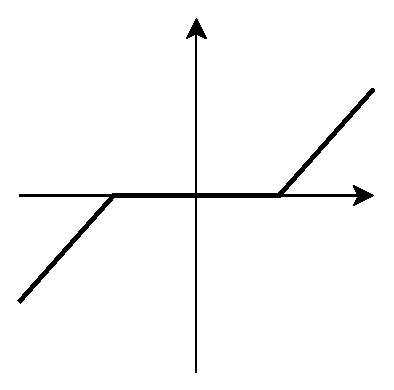
\includegraphics{func_nosense.eps} &
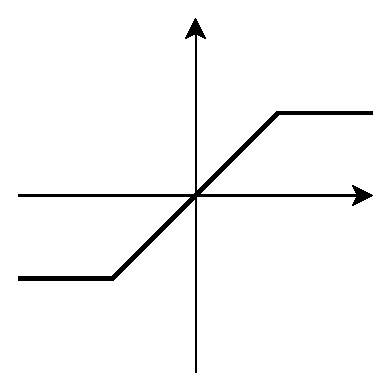
\includegraphics{func_saturat.eps} \\
а) Зона нечувствительности ({\tt nosense})& б) Насыщение ({\tt saturat}) \\
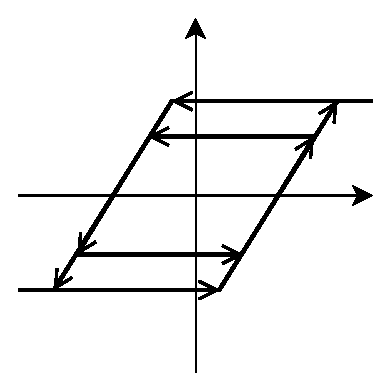
\includegraphics{func_luft.eps} &
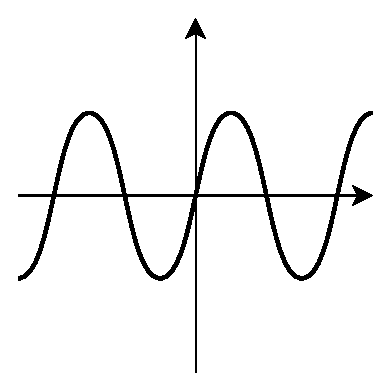
\includegraphics{func_sine.eps} \\
в) Люфт ({\tt luft}) & г) Синус ({\tt sine}) \\
\end{tabular}
\caption{Реализованные в пакете нелинейные звенья.}
\label{fig:nonlinear_functions}
\end{figure}

Количество нелинейных звеньев в пакете намеренно сделано небольшим.
Расширение списка нелинейных звеньев может быть предложено студентам в
качестве одного из направлений учебно-научной работы.

Нелинейные звенья могут комбинироваться с линейными в любом порядке.
Пример файла, задающего функцию объекта в виде инерционного звена
первого порядка $I^*(z)=\frac{1.6z}{z-0.7}$ с зоной
нечувствительности, приводится ниже:

\begin{verbatim}
;NeuCon combined function 1.0
[CombinedFunction main]
TransferFunction inert
CustomFunction deadzone

[CustomFunction deadzone]
; Extension:   .so/.dll depending the OS
file    nosense
;HalfWidth Gain
options 0.5 2
;Initial vector (may be empty)
initial

[TransferFunction inert]
polyfrac 0
 1.6 0 /  1 -0.7
\end{verbatim}

Краткое описание формата файла комбинированной функции приводится в
\tablref{tabl:cof_syntax}.

\begin{table}[ht]
\centering
\caption{Описание формата файла задания комбинированной функции.}
\label{tabl:cof_syntax}
\begin{tabular}{|c|l|p{8cm}|}
\hline
Правило & Синтаксис & Семантика \\
\hline
1 & \tt ;NeuCon combined function 1.0 & Служебный комментарий в первой строке файла \\
2 & \tt ;                    & Признак комментария до конца строки \\
3 & \tt [CombinedFunction \em Имя \tt] & Признак начала описания комбинированной функции, действующей в порядке перечисления \\
4 & \tt TransferFunction \em Имя & Ссылка на линейную функцию {\em Имя} \\
5 & \tt CustomFunction \em Имя & Ссылка на пользовательскую функцию {\em Имя} \\
6 & \tt [TransferFunction \em Имя \tt] & Признак начала описания передаточной функции (см. \tablref{tabl:tf_syntax})\\
7 & \tt [CustomFunction \em Имя \tt] & Признак начала описания пользовательской функции \\
8 & \tt file \em ИмяФайла & Имя файла без расширения ({\tt .so} или {\tt.dll}) с библиотекой, реализующей функцию \\
9 & \tt options \em Параметры & Перечень числовых параметров функции (через пробел) \\
10 & \tt initial \em Инициализация & Перечень чисел для инициализации начального состояния функции (через пробел) \\
\hline
\end{tabular}
\end{table}


\subsubsection{Нестационарные элементы моделирования}

Нестационарное поведение объектов моделирования реализуется в
программном пакете двумя способами:
\begin{enumerate}
\item с помощью специально запрограммированного звена, обладающего
  нестационарными свойствами;
\item заданием списка функций и времени переключения с одной функции
  на другую.
\end{enumerate}

Первый способ более общий.  Он позволяет реализовать произвольное
поведение объекта, например, плавное изменение параметров.  Однако он
требует запрограммировать необходимые действия и скомпилировать
полученный программный модуль в виде внешней пользовательской
библиотеки, что не всегда удобно и ведет к дополнительному расходу
времени.

Второй способ позволяет описать в текстовом файле комбинированной
функции правило, по которому будет изменяться функция объекта.
Правило задается перечнем функций и периодами времени, в которые эти
функции реализуют поведение объекта.  В целом, для функций $g_i()$ и
моментов времени $t_i$ правило вычисления действующей функции объекта
описывается формулой:

$$
y=\left\{
\begin{array}{ll}
  g_1(t,x), & 0\le t < t_1\\
  g_2(t,x), & t_1\le t < t_2\\
  ... & \\
  g_l(t,x) & t \ge t_l
\end{array}\right.
$$

\noindent где все $t_i$ кратны шагу дискретизации времен в сеансе
моделирования.

Например, если надо запрограммировать изменение коэффициента усиления
c 1.5 на 3.4 в момент времени $t=500$, это можно описать в файле
следующей комбинированной функцией:

\begin{verbatim}
;NeuCon combined function 1.0
[CombinedFunction main]
TransferFunction k1 0 500
TransferFunction k2 500 -1

[TransferFunction k1]
polyfrac 0
 1.5 /  1

[TransferFunction k2]
polyfrac 0
 3.4 /  1
\end{verbatim}

%\subsubsection{Нейронные сети и методы их обучения}
\subsubsection{Моделирование динамических систем}

Задача моделирования динамической системы в дискретном времени
заключается в упорядоченной активации взаимосвязанных функциональных
блоковб моделирующих поведение отдельных элементов системы и передачи
порций данных между ними.  Типичной динамической системой является
контур управления с обратной связью.  Входными данными для этой
системы является внешний сигнал уставки.  С целью имитации реальных
условий в контуре присутствует аддитивная помеха в канале наблюдения
объекта.  Таким образом, помеху также можно отнести к внешним
сигналам.  Остальные сигналы производятся функциональными блоками в
процессе моделирования.

Задачей программы моделирования является правильная коммутация
выходных сигналов одних функциональных блоков на вход других.  Если
принять функциональный блок за узел, а передачу данных между блоками
--- за направленное ребро, то модель динамической системы может быть
представлена как ориентированный граф.  Для обеспечения правильных
результатов моделирования и, учитывая, что оно происходит в дискретном
времени, функциональный блок должен вырабатывать порцию выходных
данных только если у него есть для этого данные на входах.  Важной
особенностью является однократное использование каждой порции данных
на входе любого блока.  Таким образом, порции данных также являются
синхронизирующими метками.  Графы описанного типа относятся к классу
сетей Петри (???), применяемых в моделировании динамических систем
различных типов.

Помимо моделирования контура управления с обратной связью описанный
аппарат сетей Петри хорошо подходит для реализации различных схем
обучения нейронных сетей как в контуре управления, так и вне его.  При
этом естественным образом выражаются многие аспекты алгоритмов
обучения нейронных сетей, такие как последовательное и пакетное
обучение, задание порядка обучающих пар, компоновка обучающих пар для
реализации нейросетевых моделей авторегрессии и скользящего среднего.
Таким образом, для решения всех основных задач, перечисленных в
п.\ref{main_tasks}, можно воспользоваться одним и тем же аппаратом.

Особенностью динамических систем, моделируемых в программном пакете,
является наличие обратной связи в контуре управления, то есть,
ориентированный граф содержит цикл.  В рамках описанного формального
подхода наличие цикла мешает начать моделирование контура управления,
поскольку в начальный момент времени для расчета ошибки управления
необходимо из уставки вычесть наблюденный на предыдущем шаге выход
объекта управления, в том время как предыдущего шага ещё нет.  Для
разрешения этой проблемы в одном из ребер цикла графа вводится
специальная порция данных --- так называемый стартёр.  Эта порция
данных представляет собой начальные условия, позволяющие запустить
нормальное функционирование контура обратной связи.

В объектно-ориентированной библиотеке {\tt NeuArch} реализован набор
унифицированных классов, позволяющих организовать в программе сеть
Петри произвольной архитектуры (не более чем с одним циклом) из
функциональных блоков, интерфейс взаимодействия между которыми
абстрагирован.  Каждый блок может иметь произвольное число входов и
выходов, причем единицей передаваемых данных является вектор ---
массив чисел зафиксированной на этапе создания сети размерности.
Имеются два основных правила, которому должны следовать все прикладные
блоки сети Петри:
\begin{enumerate}
\item функция блока активируется только если на всех входах есть
  свежие данные;
\item функция блока всегда производит свежие данные на всех выходах.
\end{enumerate}

Библиотека позволяет реализовать и более сложную логику поведения
функциональных блоков, однако пользоваться этими возможностями следует
осторожно во избежание неожиданных эффектов при моделировании.

\subsubsection{Объекты для моделирования дискретных динамических систем}

Для построения основных прикладных вычислительных программ библиотека
предлагает широкий спектр функциональных блоков, имеющих
вычислительное, коммутационное и системное назначение
(\tablref{tabl:pn_objects}).
%  Для удобства разработки программ с
%сетями Петри и лучшего понимания их функционирования разработана
%система графических обозначений для некоторого количества
%специфических блоков.  Эти блоки перечислены на~\figref{fig:pn_icons}.

\begin{table}
\centering
\caption{Функциональные блоки для построения сети Петри.}
\label{tabl:pn_objects}
\begin{tabular}{|l|l|p{11.5cm}|}
\hline
$\mathrm N^0$ & Класс \tt C++ & Назначение \\
\hline
1  & \tt NaPNActor & Заданное действие по приходу данных. \\
2  & \tt NaPNBus2i1o & Склейка двух векторных входов в один векторный выход суммарной размерности. \\
3  & \tt NaPNCheckPoint & Транзитное звено с протоколированием потока данных в заданный файл. \\
4  & \tt NaPNComparator & Вычисление разности двух входных векторов. \\
5  & \tt NaPNConstGen & Генератор постоянного значения на выходе. \\
6  & \tt NaPNCuSum & Обнаружение разладки с помощью АКС. \\
7  & \tt NaPNDelay & Формирование по входу $x_k$ выхода $x_k,x_{k-1},...,x_{k-D}$, где $D$ --- заданная задержка. \\
8  & \tt NaPNDerivative & Вычисление дискретной производной. \\
9  & \tt NaPNFetcher & Выборка некоторых элементов из входного вектора. \\
10 & \tt NaPNFill & Выдача заданного значения в качестве нескольких первых порций данных. \\
11 & \tt NaPNFileInput & Чтение данных из файла. \\
12 & \tt NaPNFileOutput & Запись данных в файл. \\
13 & \tt NaPNGenerator & Генерировать выходные значения с помощью заданной функции. \\
14 & \tt NaPNLogicalAND & Логическое ``И'' над входами.  Положительное значение --- истина ($+1$), нулевое или отрицательное --- ложь ($0$). \\
15 & \tt NaPNNNUnit & Вычисление выхода по входу нейронной сетью. \\
16 & \tt NaPNQueueInput & Чтение данных из внешнего источника общего вида. \\
17 & \tt NaPNQueueOutput & Запись данных во внешний приемник общего вида. \\
18 & \tt NaPNRandomGen & Генерация псевдослучайной последовательности. \\
19 & \tt NaPNSkip & Пропуск указанного количества первых порций данных. \\
20 & \tt NaPNStatistics & Расчет статистических параметров входных данных нарастающим итогом. \\
21 & \tt NaPNSum & Суммирование входов. \\
22 & \tt NaPNSwapper & Управляемый коммутатор прямого или перекрестного отображения входов на выходы. \\
23 & \tt NaPNSwitcher & Управляемый коммутатор направления первого или второго входа на выход. \\
24 & \tt NaPNTeacher & Обучение нейронной сети. \\
25 & \tt NaPNTrainDataGath & Сбор обучающих данных по критерию минимальной плотности покрытия. \\
26 & \tt NaPNTimeDepend & Счетчик дискретного времени. \\
27 & \tt NaPNTimer & Счетчик тактов моделирования. \\
28 & \tt NaPNTransfer & Передаточная функция. \\
29 & \tt NaPNTrigger & Управляемый пропуск порций данных. \\
30 & \tt NaPNWatcher & Заданное действие над порцией данных.\\
\hline
\end{tabular}
\end{table}

%\begin{figure}[h]
%\centering
%\begin{tabular}{cс}
%\hbox{\input{Bus2i1o.pic}} & \hbox{\input{Comparator.pic}} \\
%а) & б)\\
%\end{tabular}
%\caption{Графические обозначения некоторых функциональных блоков: (а)
%         и рабочего функционирования (б).}
%\label{fig:pn_icons}
%\end{figure}

%Bus2i1o.pic
%Comparator.pic
%Summator.pic
%Delay.pic
%Delta.pic
%FetcherLtoR.pic
%FileIO.pic
%LAnd.pic
%QueueL.pic
%QueueR.pic
%RandomNormal.pic
%RandomUniform.pic
%Skip.pic
%Statistics.pic
%SwitcherPM.pic
%TriggerLtoR.pic
%NNUnit.pic
%Teacher.pic
%
%\subsubsection{Формализм для графического представления динамических моделей}
%\subsubsection{Пример: дообучение нейросетевого регулятора в контуре}
%\subsubsection{Пример: моделирование САУ и обнаружение разладки}
